\subsection{Bathymetry}
\label{sec: bathy}

	Survey data collected on October 1st was considered for this analysis. These data were measured via the CRAB and a Trimble Real Time Kinematic (RTK) GPS system. Elevation data from six cross-sections\footnote{we could potentially add an overhead plot of the transects}, perpendicular to the shoreline, spaced over a 100 meter portion of the beach were combined to create the 2D surface shown below in Figure \ref{2D Bath}. 
	
	 	\begin{figure}[H]
	 	\centering
	 	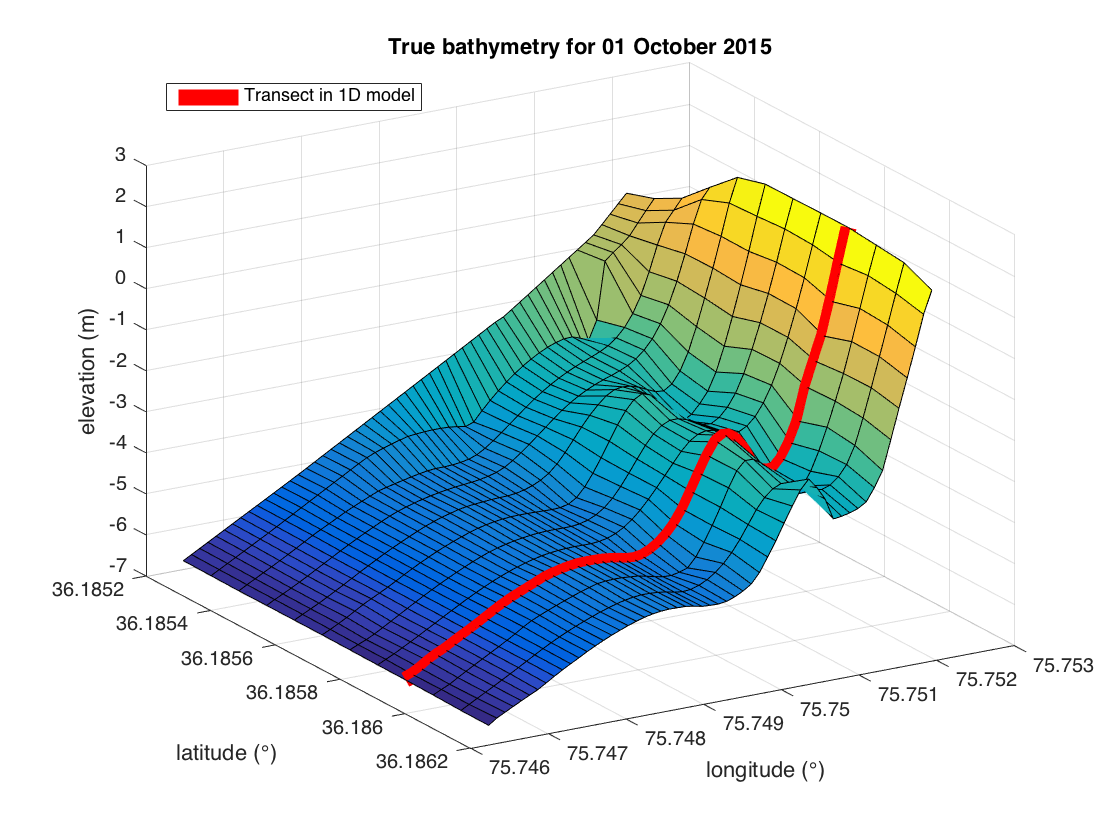
\includegraphics[width=0.6\linewidth]{img/trueBath2D.png}
	 	\caption{2D Bathymetry}
	 	\label{2D Bath}
	 	\end{figure}
	
	For the 1D problem, a single slice of the 2D bathymetry was used as model input, identified by the red line in Figure \ref{2D Bath}. In a cartesian co-ordinate system, this line (a.k.a 'transect') is located at y = 950 meters. 
		
		\begin{figure}[H]
		\centering
		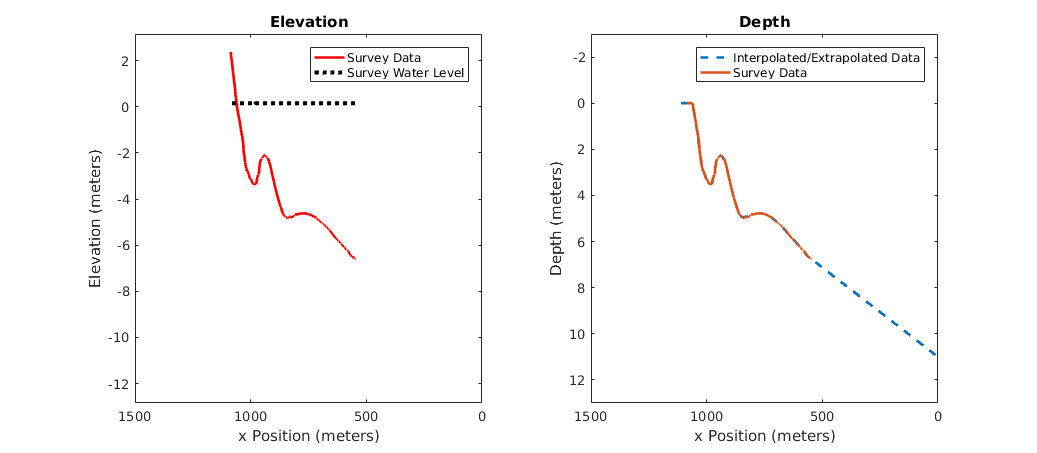
\includegraphics[width = 1.0\linewidth]{img/trueBath1D.png}
		\caption{1D Bathymetry - elevation data (left) and depth data (right).}
		\label{1D Bath}
		\end{figure}
		
	Survey data provided sea floor elevation referenced to the North American Vertical Datum of 1988 (NAVD88) (Figure \ref{1D Bath} \textit{left}). To provide proper input data for the 1D model, elevation needed be transformed to depth data (Figure \ref{1D Bath} \textit{right}). Once transformed, depth is discretized by interpolating between measured data points via Matlab's built in pchip method. Pchip was chosen for the interpolation method due to its shape preserving nature as to not introduce non-physical oscillations. Between the boundary condition and the nearest measured depth point linear interpolation was used to fill in missing data.